\documentclass{article}

\usepackage[usenames]{color}
\usepackage{graphicx}
\usepackage{amsmath}
\usepackage{amsfonts}
\usepackage{amssymb}
\usepackage{mathrsfs}
\usepackage{bm}
\usepackage{verbatim}
\usepackage{cancel}

\begin{document}

\begin{figure}[htbp]

%\centering
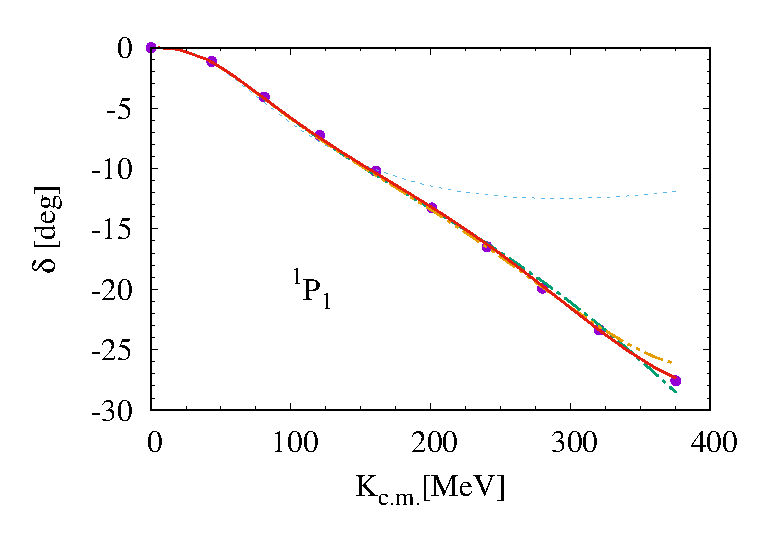
\includegraphics[width=0.5\textwidth]{7_1p1.eps}
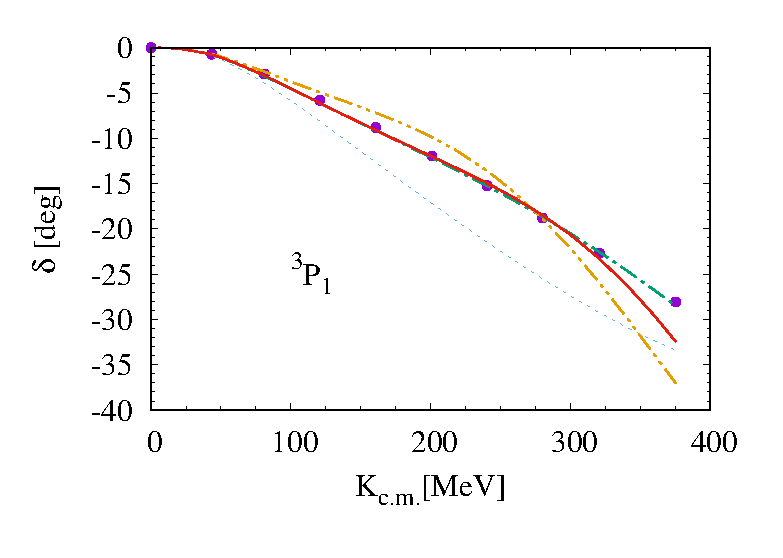
\includegraphics[width=0.5\textwidth]{7_3p1.eps}
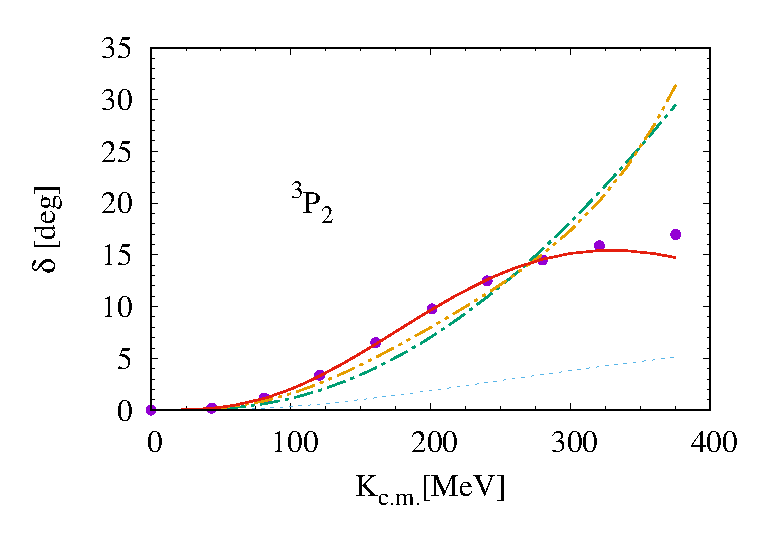
\includegraphics[width=0.5\textwidth]{7_3p2.eps}
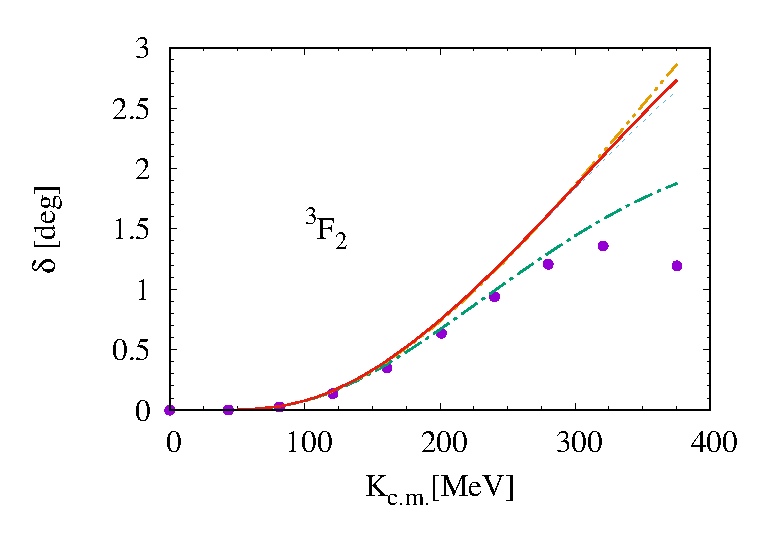
\includegraphics[width=0.5\textwidth]{7_3f2.eps}
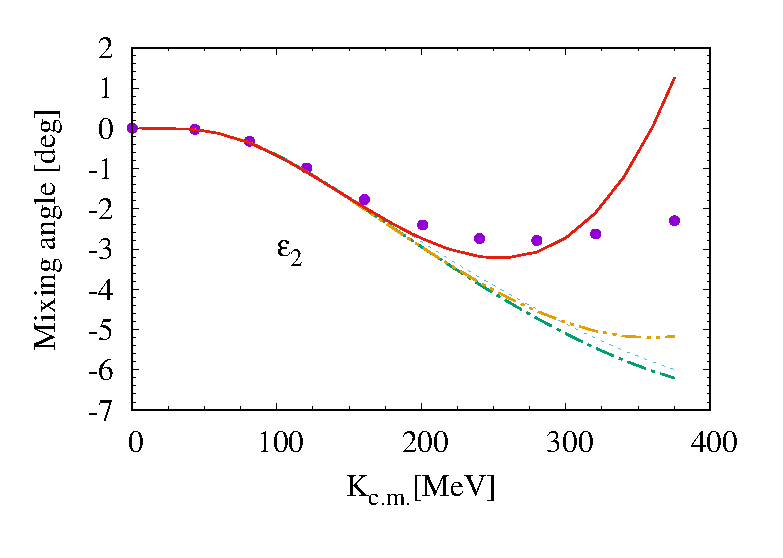
\includegraphics[width=0.5\textwidth]{7_e2.eps}
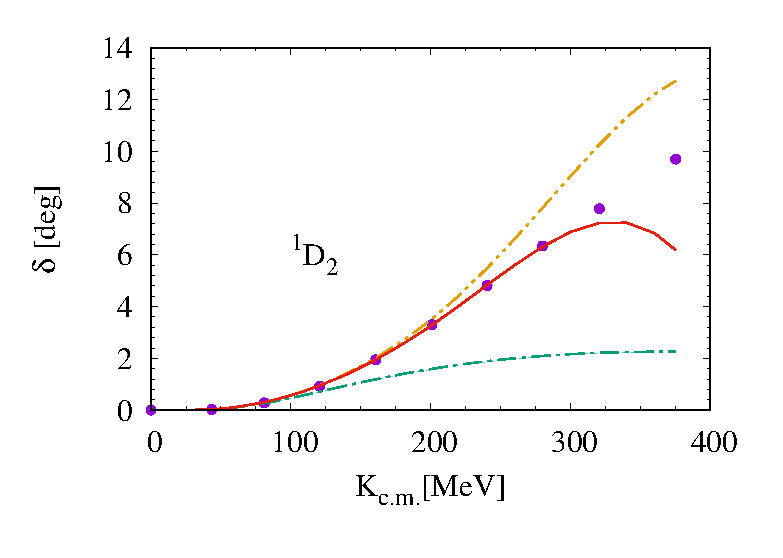
\includegraphics[width=0.5\textwidth]{7_1d2.eps}
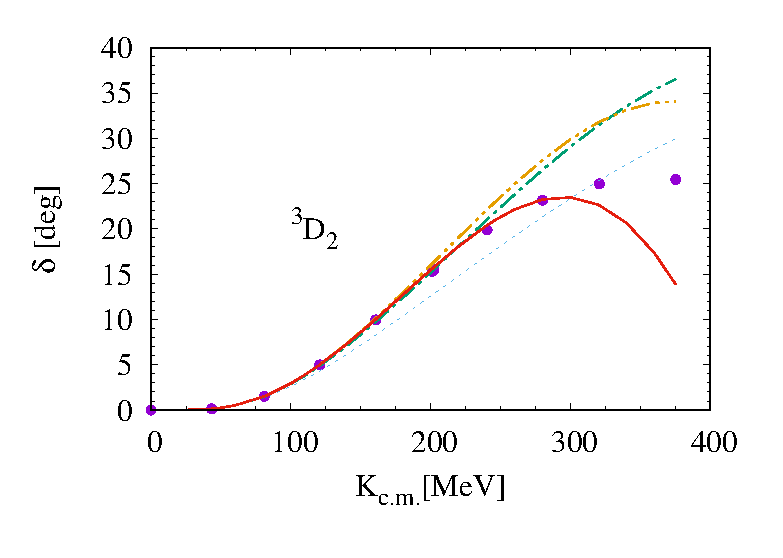
\includegraphics[width=0.5\textwidth]{7_3d2.eps}
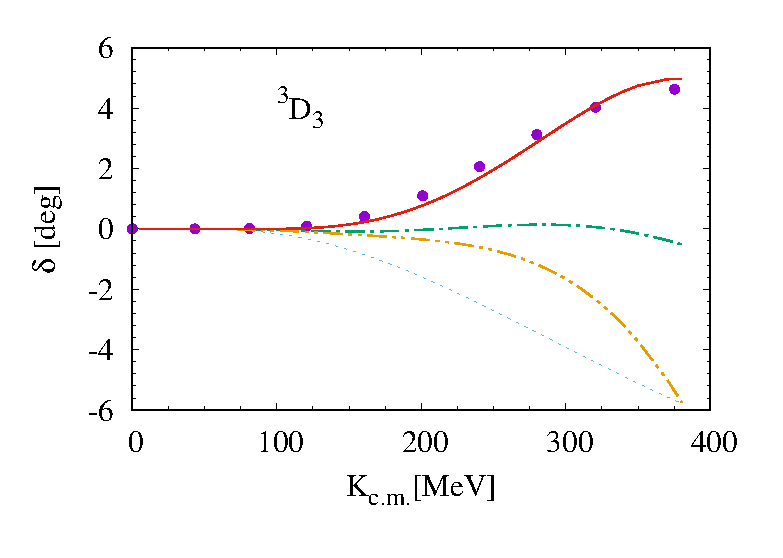
\includegraphics[width=0.5\textwidth]{7_3d3.eps}
\end{figure}
%\newpage
%\pagebreak[2]
\begin{figure}[htbp]
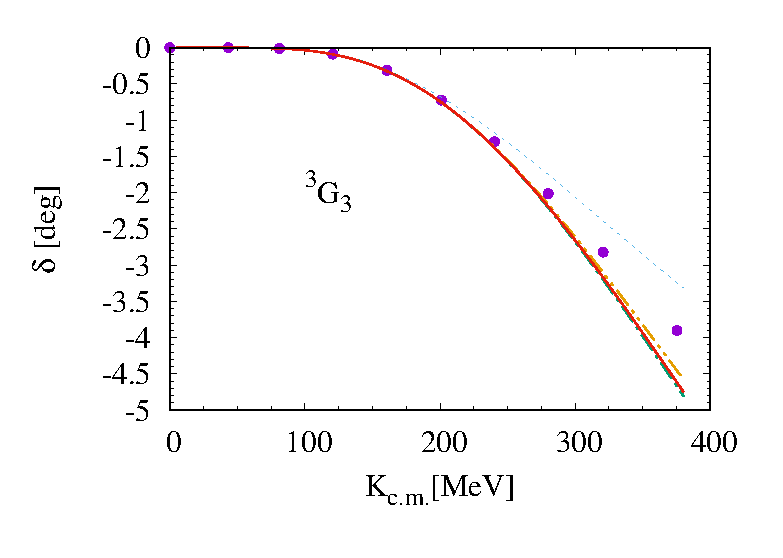
\includegraphics[width=0.5\textwidth]{7_3g3.eps}
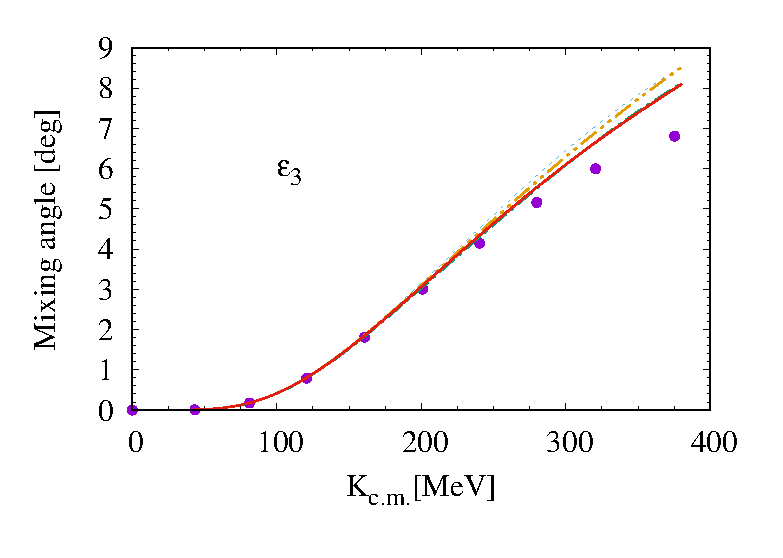
\includegraphics[width=0.5\textwidth]{7_e3.eps}
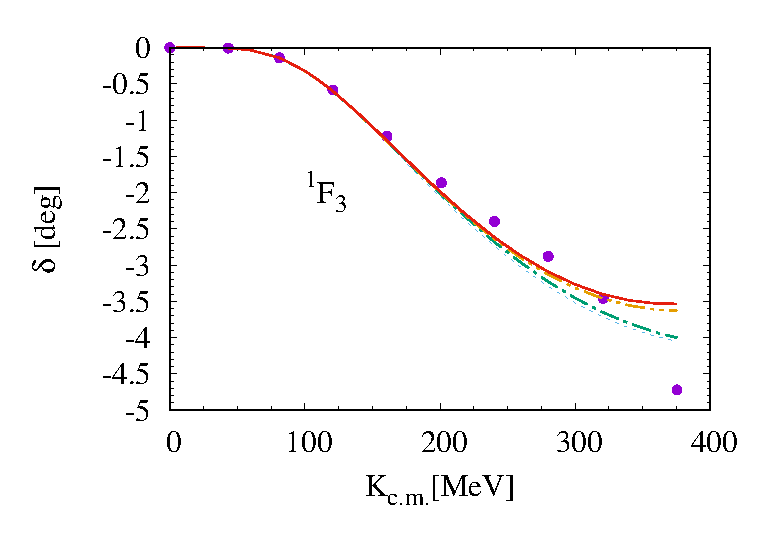
\includegraphics[width=0.5\textwidth]{7_1f3.eps}
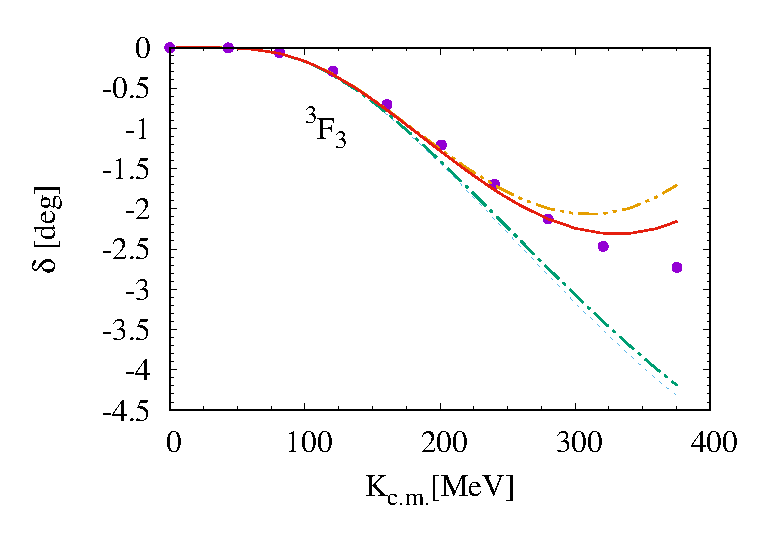
\includegraphics[width=0.5\textwidth]{7_3f3.eps}
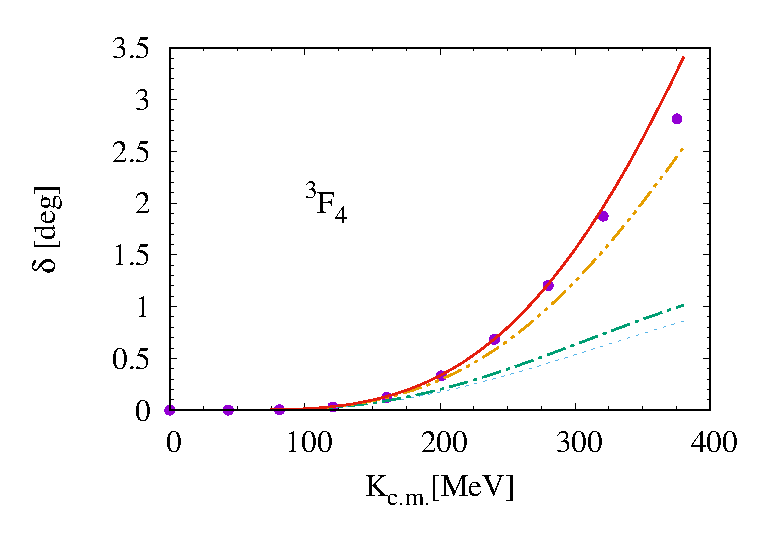
\includegraphics[width=0.5\textwidth]{7_3f4.eps}
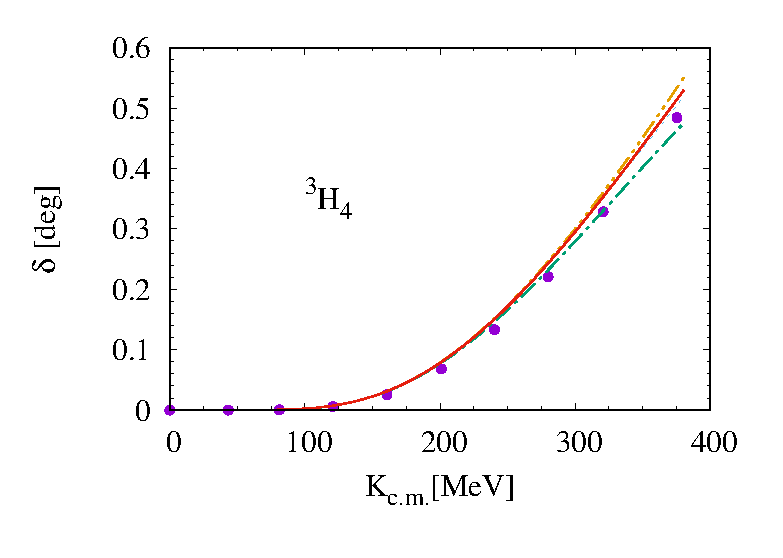
\includegraphics[width=0.5\textwidth]{7_3h4.eps}
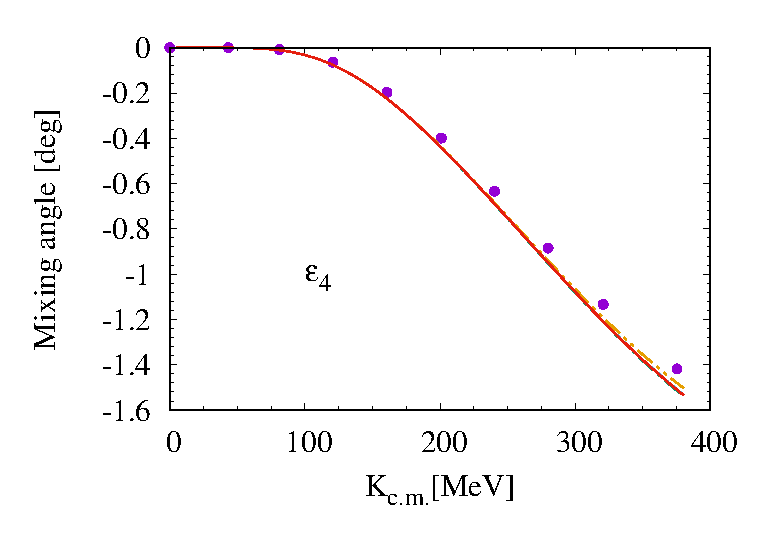
\includegraphics[width=0.5\textwidth]{7_e4.eps}
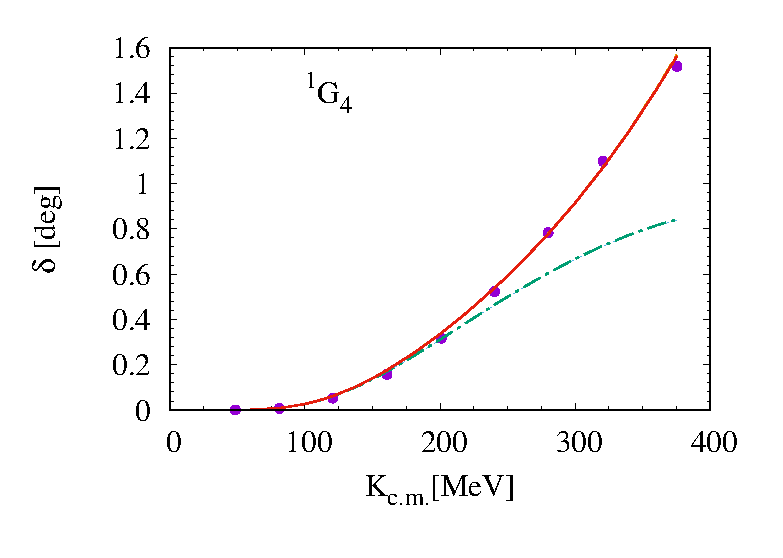
\includegraphics[width=0.5\textwidth]{7_1g4.eps}
\end{figure}
\begin{figure}[htbp]
% \label{fig:digit}
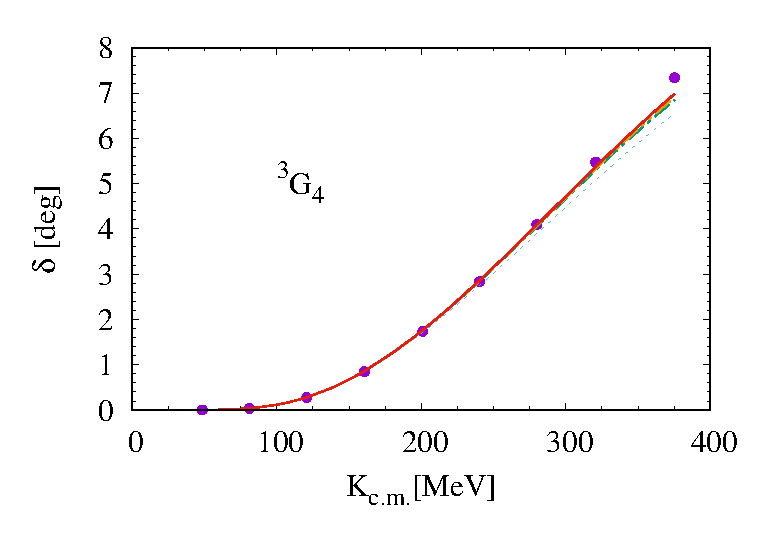
\includegraphics[width=0.5\textwidth]{7_3g4.eps}
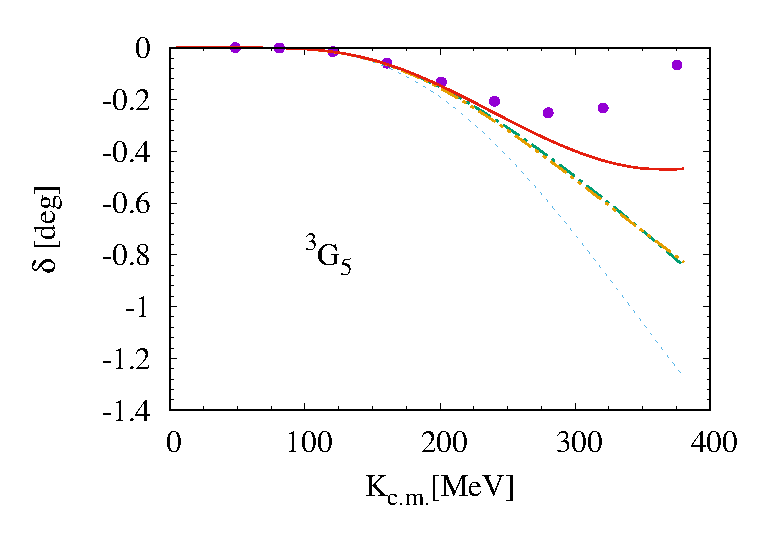
\includegraphics[width=0.5\textwidth]{7_3g5.eps}
\caption{The bule, green, orange, and red lines correspond respectively to NLO, N$^2$LO, N$^3$LO, and N$^4$LO. }
\end{figure}

\end{document}